% !Mode:: "TeX:UTF-8"
%% 请使用 XeLaTeX 编译本文. 默认使用 Adobe 字体. 需自行安装.
\documentclass{whuBSthesis}% 选项 forprint: 交付打印时添加, 避免彩色链接字迹打印偏淡. 即使用下一行:
%\documentclass[forprint]{whuBSthesis}

%%% --- 下面 4 个宏包是为了本文中的一些例子. 与模板本身无关, 实际使用中建议删除.】
\usepackage{cases}    % 分段函数表达式, 每个式子加编号. 本文中有例子.
\usepackage{fvrb-ex} % 是为了书写本文第二章的例子: 右边是源码, 左边是结果.
\usepackage{everb}   % 本文中的 everbatim 环境, \everb 等命令就来自此宏包.
                            \everbsetup{box=false, bgcolor={[rgb]{0.92,0.92,1.00}}} % everb 包中的命令, 设置边框, 背景.
\usepackage{dtklogos}  % TeX\LaTeX 的各种常用 logo.
%%% --- 上述 4 个宏包, 实际使用中建议删除.

%%%--- 数学符号申明 %%%%%%%%%%%%%%%%%%%%%%%%%%%%%%%%
\DeclareMathOperator{\arccot}{arccot}  % 是为了说明文中的一个例子. 【与模板本身无关, 实际使用中可以删除.】


%%===参考文献===%%%%%%%%%%%%%%%%%%%%%%%%%%%%%%%%
\bibliographystyle{abbrv}        % 参考文献样式,  plain,unsrt,alpha,abbrv,chinesebst 等等
%%%%%%%%%%%%%%%%%%%%%%%%%%%%%%%%%%%%%%%%%%%
\graphicspath{{figures/}}        % 图片文件路径
%%%%%%%%%%%%%%%%%%%%%%%%%%%%%%%%%%%%%%%%%%%
\allowdisplaybreaks
%%%%%%%%%%%%%%%%%%%%%%%%%%%%%%%%%%%%%%%%%%%

\begin{document}
%%%%%%% 下面的内容, 据实填空.

\miji{ }                                      % 密级. 没有就空着.
\StudentNumber{2010123456789} % 填写自己的学号

\title{武汉大学本科毕业论文~\LaTeX~模板}
\Etitle{A \LaTeX~Thesis Template for Wuhan University} % 英文题目
\author{黄正华}                            % 作者名字
\Eauthor{HUANG Zhenghua}            %作者英文名
\Csupervisor{胡宝清\quad 教授}        %指导教师中文名、职称
\Esupervisor{Prof.~HU Bao Qing}     %指导教师英文名、职称
\Cmajor{信息与计算科学}                  % 专业中文名
\Emajor{Information and Computing Science}% 专业英文名
\Cschoolname{数学与统计学院}          % 学院名
\Eschoolname{School of Mathematics and Statistics} %学院英文名. 不确定的话, 请看一下自己学院的网页上是怎么写的. 别搞错了!
\date{二〇一四年六月}                    % 日期, 要注意和英文日期一致!!
\Edate{June, 2014}                       % 英文封面日期










%-----------------------------------------------------------------------------
\pdfbookmark[0]{封面}{title}         % 封面页加到 pdf 书签
\maketitle
\frontmatter
\pagenumbering{Roman}              % 正文之前的页码用大写罗马字母编号.
%-----------------------------------------------------------------------------
% !Mode:: "TeX:UTF-8"

%%% 此部分需要自行填写: (1) 中文摘要及关键词 (2) 英文摘要及关键词
%%%%%%%%%%%%%%%%%%%%%%%%%%%%%
%%% -------------  英文封面 (无需改动)-------------   %%%
%%%%%%%%%%%%%%%%%%%%%%%%%%%%%
\thispagestyle{empty}
\renewcommand{\baselinestretch}{1.5}  %下文的行距
\vspace*{0.5cm}
\begin{center}
{\Large \bf BACHELOR'S DEGREE THESIS \\[1ex] OF WUHAN UNIVERSITY }
\end{center}
\vspace{2.5cm}
\begin{center}{\zihao{2} \the\Etitle \par}\end{center}

\vfill

\begin{center}
\zihao{4}
\begin{tabular}{ r l }
 School (Department): & {\sc \the\Eschoolname}\\
  Major:          &   {\sc\the\Emajor}  \\
 Candidate:      &  {\sc \the\Eauthor}      \\
 Supervisor:     &  {\sc \the\Esupervisor}
\end{tabular}

\vspace*{2cm}
\begin{center}
   \ifprint % 文档打印, 使用黑白校徽.
  
\includegraphics[height=4cm]{whu.eps}       %%  黑白的.
  \else
  
\includegraphics[height=4cm]{whulogo.eps} %%  彩色的.
  \fi
\end{center}


\zihao{-2}
%\the\Schoolname\\
{\sc Wuhan University}

\vspace*{1.0cm}

\the\Edate

\end{center}
%%% 郑重声明部分无需改动

%%%---- 郑重声明 (无需改动)------------------------------------%
\newpage
\vspace*{20pt}
\begin{center}{\ziju{0.8}\zihao{-2}\ttfamily\bfseries 郑重声明}\end{center}
\par\vspace*{30pt}
\renewcommand{\baselinestretch}{2}
{\zihao{4}%

本人呈交的学位论文, 是在导师的指导下, 独立进行研究工作所取得的成果,
所有数据、图片资料真实可靠. 尽我所知, 除文中已经注明引用的内容外,
本学位论文的研究成果不包含他人享有著作权的内容.
对本论文所涉及的研究工作做出贡献的其他个人和集体,
均已在文中以明确的方式标明. 本学位论文的知识产权归属于培养单位.\\[2cm]

\hspace*{1cm}本人签名: $\underline{\hspace{3.5cm}}$
\hspace{2cm}日期: $\underline{\hspace{3.5cm}}$\hfill\par}
%------------------------------------------------------------------------------
\baselineskip=23pt  % 正文行距为 23 磅
%------------------------------------------------------------------------------





%%======中文摘要===========================%
\begin{cnabstract}
本文主要介绍和讨论了武汉大学本科毕业论文的~\LaTeX~模板.
指明了编译方法, 强调了公式排版的一些细节问题, 也指出了一些常见的排版错误.



\end{cnabstract}
\par
\vspace*{2em}


%%%%--  关键词 -----------------------------------------%%%%%%%%
%%%%-- 注意: 每个关键词之间用“;”分开,最后一个关键词不打标点符号
\cnkeywords{毕业论文; \LaTeX{}; 模板; \XeLaTeX{}}


%%====英文摘要==========================%


\begin{enabstract}
This thesis is a study on the theory of \dots.

\end{enabstract}
\par
\vspace*{2em}

%%%%%-- Key words --------------------------------------%%%%%%%
%%%%-- 注意: 每个关键词之间用“;”分开,最后一个关键词不打标点符号
 \enkeywords{\LaTeX{}; \XeLaTeX{}}
    % 加入摘要, 申明.
%==========================把目录加入到书签==============================%%%%%%
\pdfbookmark[0]{目录}{toc}
\tableofcontents
\mainmatter %% 以下是正文
%%%%%%%%%%%%%%%%%%%%%%%%%%%--------main matter-------%%%%%%%%%%%%%%%%%%%%%%%%%%%%%%%%%%%%
\chapter{先说重要的}
 
\section{具体使用步骤}
\begin{description}
  \item[Step 0]  安装 Adobe 字体. 具体见 \ref{sec-Adobe} 节.
  \item[Step 1]  进入 includefile 文件夹,  打开 frontmatter.tex, backmatter.tex 这两个文档,
        分别填写 (1) 中文摘要、英文摘要, (2) 致谢.

  \item[Step 2]  打开主文档 WHU-B.S.-template.tex, 填写题目、作者等等信息, 书写正文.

  \item[Step 3]  使用 \XeLaTeX{} 编译. 具体见 \ref{sec-compile} 节.


\end{description}



\section{安装字体}\label{sec-Adobe}

需要安装 Adobe 字体.

{\kaishu 本文默认使用 Adobe 字体. 字体文件已经在 Adobe fonts 文件夹里.

安装很简单: 鼠标右键点击字体文件, 弹出的菜单中点击安装即可.

优点: 字迹清晰、悦目. 强烈推荐使用 Adobe 字体.

若您不想使用 Adobe 字体的话, whuBSthesis.cls 的第4行去掉选项 adobefonts. }


\section{编译的方法}\label{sec-compile}

默认使用 \XeLaTeX{} 编译.

若另存为新文档, 必须选择文档保存类型为 \verb|:UTF-8|.

{\kaishu 可能因习惯使然, 有的朋友不太接受新的编译方式.
其实 \LaTeX{} 一直在发展变化中, 我们可以尝试新方法带给我们的便利.
我个人使用的编译方式也都是从 \LaTeX{}, CCT,  pdf\LaTeX{}, \XeLaTeX{} 一点点过来的. }

使用~\XeLaTeX{} 编译, 直接生成~pdf 文件.
pdf 文件也可以反向搜索! {\CJKunderwave{双击~pdf 中要修改的文字, 将直接跳转到源文件中相应位置}}.
这个是由~Sumatra PDF 软件实现的.

Sumatra PDF 是一个~pdf 阅读器. CTeX 2.9 套装已经集成了~Sumatra PDF, 预览时将默认使用~Sumatra PDF 查看编译结果.



\section{文档类型选择}
文档类型有 2 种情形:

\begin{table}[ht]\centering
\begin{tabular}{ll}
\hline
   \verb|\documentclass{whuBSthesis}|                   &  毕业论文 \\
   \verb|\documentclass[forprint]{whuBSthesis}|        &  毕业论文打印版 \\
\hline
\end{tabular}
\end{table}
相关解释见下节.


\section{打印的问题}
\begin{enumerate}[i)]
  \item  论文要求\colorbox{yellow}{单面打印}.
  \item  关于文档选项 forprint: 交付打印时, 建议加上选项 forprint, 以消除链接文字之彩色, 避免打印字迹偏淡.
  \item  打印时留意不要缩小页面或居中. 即页面放缩方式应该是``无''(Adobe Reader XI 是选择``实际大小'').
           有可能页面放缩方式默认为``适合可打印区域'', 会导致打印为原页面大小的 $97\%$.
           文字不要居中打印, 是因为考虑到装订, 左侧的空白留得稍多一点(模板已作预留).
  \item  遗留问题: 封面需要打印部重新制作.  校内打印部通常有现成的模板.
           我们自己做的封面, 打印部不一定好用.
\end{enumerate}
%如果不是彩色打印机, 请在打印时, 选择将彩色打印为黑白, 否则彩色文字打出的墨迹会偏淡.


 \vfill

本文档下载更新地址: \url{http://aff.whu.edu.cn/huangzh/}. 使用之前, 请移步查看是否有更新.

问题反馈及建议, 请联系: huangzh@whu.edu.cn.



\chapter{杂七杂八的话}

\section{Readme}

模板文件的结构, 如下表所示:
 \begin{table}[ht]\centering
\begin{tabular}{r|r|l}
\hline\hline
  \multicolumn{2}{l|}{WHU-B.S.-template.tex }  &  主文档. 在其中填写正文.\\ \hline
  \multicolumn{2}{l|}{whuBSthesis.cls } &  定义文档格式的 class file. 不可删除.\\ \hline
                          &frontmatter.tex&   郑重声明、中英文摘要. \\ \cline{2-3}
 \raisebox{1em}{includefile 文件夹}  & backmatter.tex &  致谢.  \\ \hline
  \multicolumn{2}{l|}{Adobe fonts 文件夹}  &  Adobe 字体文件, 需自行安装.\\ \hline
  \multicolumn{2}{l|}{figures 文件夹} &  存放图片文件.\\ \hline\hline
\end{tabular}
\end{table}

无需也不要改变、移动上述文档的位置.

如果不习惯用~\verb|\include{ }|~的方式加入``子文档'', 当然可以把它们合并在主文档, 成为一个文档.
({\kaishu 但是这样并不会给我们带来方便.})

利用~WinEdt~的~Project tree, 可以方便地管理这些文件:
\begin{itemize}
    \item 点击~WinEdt~窗口的~Project Tree~按键;
    \item 再点击~WinEdt~窗口的~Set Main File~按键;
\end{itemize}
接下来的管理, 已经清楚地展示在跳出的窗口中了. 再去处理其他的文件时, 还要点击~\WinEdt~窗口的~Remove Main File~按键.

2013 年 12 月更新: 文件夹下放了一个 ntheorem.sty. 是因为有用户遇到了不能编译的问题, 其原因就是需要更新 ntheorem.sty.
若你知道更新的方法, 感觉这个碍眼, 可以把这个文件去掉. 不知道更新的方法, 就这样放在这里吧.

2013 年 12 月更新: 加上英文封面. 教务部的写作规范中的附例, 并没有英文封面. 但是遇到很多同学说要加上.

2014 年 05 月更新: 参考文献加到目录. 感谢武汉大学计算机学院孙启航同学、数学与统计学院李振坤同学指出这个纰漏.

2014 年 06 月更新: 修改章节标题、声明标题、图表标题的字体和大小. 再次感谢孙启航同学.

 \section{字体调节}

\begin{tabular}{ll}
 \verb|\songti| & {\songti 宋体} \\
 \verb|\heiti| & {\heiti 黑体} \\
 \verb|\fangsong| & {\fangsong 仿宋} \\
 \verb|\kaishu| & {\kaishu 楷书}
\end{tabular}


\section{字号调节}
字号命令: \verb|\zihao| \index{zihao}

\begin{tabular}{ll}
\verb|\zihao{0}| &\zihao{0}  初号字 English \\
\verb|\zihao{-0}|&\zihao{-0} 小初号 English \\
\verb|\zihao{1} |&\zihao{1}  一号字 English \\
\verb|\zihao{-1}|&\zihao{-1} 小一号 English \\
\verb|\zihao{2} |&\zihao{2}  二号字 English \\
\verb|\zihao{-2}|&\zihao{-2} 小二号 English \\
\verb|\zihao{3} |&\zihao{3}  三号字 English \\
\verb|\zihao{-3}|&\zihao{-3} 小三号 English \\
\verb|\zihao{4} |&\zihao{4}  四号字 English \\
\verb|\zihao{-4}|&\zihao{-4} 小四号 English \\
\verb|\zihao{5} |&\zihao{5}  五号字 English \\
\verb|\zihao{-5}|&\zihao{-5} 小五号 English \\
\verb|\zihao{6} |&\zihao{6}  六号字 English \\
\verb|\zihao{-6}|&\zihao{-6} 小六号 English \\
\verb|\zihao{7} |&\zihao{7}  七号字 English \\
\verb|\zihao{8} |&\zihao{8}  八号字 English \\
\end{tabular}

\section{已加入的常用宏包}

\begin{description}
%  \item[amsmath,amssymb]
  \item[cite]  参考文献引用, 得到形如 [3-7] 的样式.
  \item[color,xcolor]  支持彩色.
  \item[enumerate]  方便自由选择 enumerate 环境的编号方式. 比如

  \verb|\begin{enumerate}[(a)]| 得到形如 (a), (b), (c) 的编号.


  \verb|\begin{enumerate}[i)]| 得到形如 i), ii), iii) 的编号.

\end{description}

另外要说明的是,  itemize, enumerate, description 这三种 list 环境, 已经调节了其间距和缩进,
以符合中文书写的习惯.

\section{标点符号的问题}

建议使用半角的标点符号, 后边再键入一个空格. 特别是在英文书写中要注意此问题!

双引号是由两个左单引号、两个右单引号构成的: \everb|``  ''|. 左单引号在键盘上数字~1 的左边.

但是, 无论您偏向于全角或半角, 强烈建议您使用实心的句号, 只要您书写的是自然科学的文章.
原因可能是因为, 比如使用全角句号的句子结尾处的``$x$。''容易误为数学式~$x_0$(\everb|$x_0$|)吧.



\section{引用的问题}


\subsection{参考文献的引用}

参考文献的引用, 用命令~\verb|\cite{ }|. 大括号内要填入的字串, 是自命名的文献条目名.

比如, 通常我们会说:
\begin{colorboxed}
关于什么什么问题, 我们可以参见文献 \cite{r2}. 作者某某还提到了某某概念\upcite{r1}, 等等.
\end{colorboxed}
上文使用的源文件为:
\begin{colorboxed}
关于什么什么问题, 我们可以参见文献~\verb|\cite{r2}|. 作者某某还提到了某某概念~\verb|\upcite{r1}|, 等等.
\end{colorboxed}
其中~\verb|\upcite| 是自定义命令, 使参考文献引用以上标形式出现.

({\heiti 注意:}~{\kaishu 这里文献的引用, 有时需要以上标形式出现, 有时需要作为正文文字出现, 为什么?})

另外, 要得到形如~\cite{r1,r3,r4,r5} 的参考文献连续引用, 需要在导言区引用~cite 宏包,
在正文中使用~\verb|\cite{r1,r3,r4,r5}| 的引用形式即可.
或者, 连续引用的上标形式: 使用~\verb|\upcite{r1,r2,r3}|, 得到\upcite{r1,r2,r3}.

\subsection{定理和公式的引用}

\begin{theorem}[谁发现的]\label{th-abcd}
最大的正整数是~$1$.
\end{theorem}

\begin{proof}
要找到这个最大的正整数, 我们设最大的正整数为~$x$, 则~$x \geqslant 1$, 两边同时乘以~$x$, 得到
\begin{equation}\label{eq-abc}
x^2 \geqslant x.
\end{equation}
而~$x$ 是最大的正整数, 由~\eqref{eq-abc} 式得到
\[
x^2 = x.
\]
所以
\begin{equation*}
x = 1.
\end{equation*}
\end{proof}

定理~\ref{th-abcd} 是一个重大的发现.

%%%%----- 定义等环境的举例 --------
\begin{definition}[整数]
 正整数(例如 1, 2, 3)、负整数(例如 ${−1}$, $−2$, $−3$)与零(0)合起来统称为{\heiti 整数}.
\end{definition}

\begin{remark}
  整数集合在数学上通常表示为 $\mathbf{Z}$ 或 $\mathbb{Z}$, 该记号源于德语单词 Zahlen(意为``数'')的首字母.
\end{remark}

\begin{proposition}
任意两个整数相加、相减、相乘的结果, 仍然是整数.
\end{proposition}

\begin{example}
  $1+2=3$.
\end{example}

\begin{corollary}
   在整数集合内, 相加、相减、相乘运算是封闭的.
\end{corollary}

\section{图形与表格}

支持对~eps, pdf, jpg 等等常见图形格式.

再次{\colorbox{red!45}{澄清一个广为流传的误会}}: \LaTeX{} 支持的图形格式绝非 eps 这一种. 无需特意把图片转化为 eps.

用形如~\verb|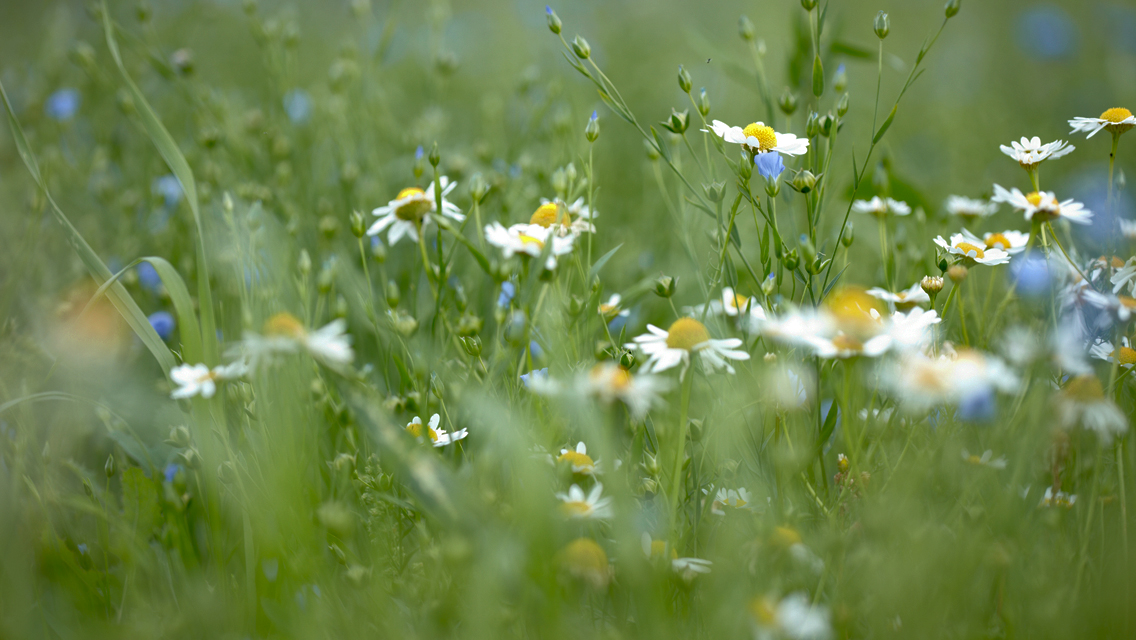
\includegraphics[width=12cm]{Daisy.jpg}| 的命令可以纳入图片.

如图~\ref{fig:1} 是一个纳入~jpg 图片的例子.

\begin{figure}[ht]
\centering
  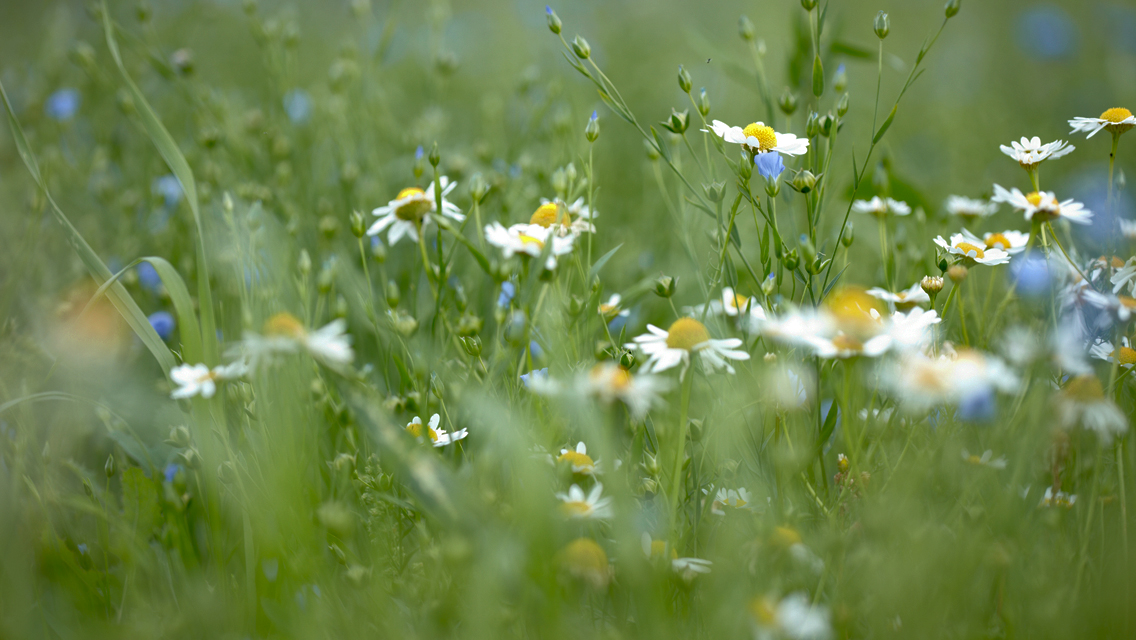
\includegraphics[width=\textwidth]{Daisy.jpg}
  \caption{一个彩色 jpg 图片的例子}
  \label{fig:1}
\end{figure}

表格问题, 建议使用``三线表'', 如表 \ref{tab:1}.

\begin{table}[ht]
\centering
\caption{一般三线表}
\label{tab:1}
    \begin{tabular}{c c c c c c c c c c c}
    \hline
    123 & 4  & 5  & 123 & 4 & 5123 & 4 & 5 & 123 & 4 & 5\\
    \hline
    67 & 890 & 13 & 123 & 4 & 5123 & 4 & 5 & 123 & 4 & 5\\
    67 & 890 & 13 & 123 & 4 & 5123 & 4 & 5 & 123 & 4 & 5\\
    67 & 890 & 13 & 123 & 4 & 5123 & 4 & 5 & 123 & 4 & 5\\
    \hline
    \end{tabular}
\end{table}



\section{如何查找说明文档}
附带说一个问题: 如何查找说明文档?
 \begin{enumerate}
    \item  在~\WinEdt{} 窗口点击进入~help~$\dashrightarrow$~LaTeX~Doc, 输入宏包名查找.
           也可以: Shift+Ctrl+F1, 填入宏包名搜索即可. ({\kaishu 马上试一下: 查找~hyperref 宏包的说明文档.})
    \item 有时间的话, 自己到安装目录下去翻看吧, 里面有无尽的宝藏.
    \item 使用万能的~Google.
\end{enumerate}
%%%============================================================================================================%%%
\chapter{公式排版的注意事项}

数学公式的排版, 建议尽可能考虑使用~amsmath 宏包.
\AMSLaTeX 在数学公式的处理上更为专业和地道.
名著``The \LaTeX{} Companion''的``Chapter 8: Higher Mathematics''简单明了地叙述了~\AMSLaTeX 的用法, 值得我们研读.
如果您安装了~CTeX 2.8 以上的套装, 目录~\everb|C:\CTEX\CTeX\ctex\doc|下名为~ch8 的~pdf 文件就是.
(点击开始 --- 所有程序 --- CTeX --- help 也可以看到. Win8 直接点击搜索即可看到该 pdf 文档, 不过此时名字显示为 Mathematics.)


另外一个示例丰富的必备文档是``Mathmode''\upcite{r5}, 作者~Herbert Vo\ss, 可以在这个网址获得:
\url{http://www.tex.ac.uk/ctan/info/math/voss/mathmode/Mathmode.pdf}.


\section{公式编号的问题}

下文要提及的~align, split, subequations, cases 等环境, 均需要调用~amsmath 宏包.
这个几乎是必用的宏包, 已在~whuBSthesis.cls 中加入了.

1. 多行公式建议使用~align 环境. 用~eqnarray 的话, 等号\footnote{当然包括不等号的情形, 以下皆同.}两侧的间距有点过大.
比较:

\begin{SideBySideExample}[xrightmargin=8cm,frame=single ]
  \begin{align}
   x+y+z&=a,\\
   1+2+3&=b.
  \end{align}
\end{SideBySideExample}

\begin{SideBySideExample}[xrightmargin=8cm,frame=single ]
  \begin{eqnarray}
   x+y+z&=&a,\\
   1+2+3&=&b.
  \end{eqnarray}
\end{SideBySideExample}


2. 多个等号需要换行的公式, 建议使用~split 环境({\kaishu 当然, 用~align 也可以}).
有的朋友在这里使用的是~eqnarray, 效果不能令人满意.

\begin{SideBySideExample}[xrightmargin=8cm,frame=single ]
  \begin{eqnarray}
    f(x) &=& x+y+z \notag\\
         &=& 1+2+3.
  \end{eqnarray}
\end{SideBySideExample}

\begin{SideBySideExample}[xrightmargin=8cm,frame=single ]
  \begin{equation}
  \begin{split}
    f(x) &= x+y+z\\
         &= 1+2+3.
  \end{split}
  \end{equation}
\end{SideBySideExample}


看看~align 的例子:
\begin{everbatim}
\begin{align}
   f(x)&=x+y+z \notag\\
       &=1+2+3.
\end{align}
\end{everbatim}
排版的结果如下:
\begin{colorboxed}[width=\linewidth]
\begin{align}
   f(x)&=x+y+z \notag\\
       &=1+2+3.
\end{align}
\end{colorboxed}
所以, align 环境的使用范围是很广的. align 环境可以``通杀''各种情形.

如果您需要在使用~split 环境时, 公式编号标在最后一行, 则需要在引用~amsmath 宏包时,
增加~tbtags 选项. 即: \everb|\usepackage[tbtags]{amsmath}|.

3.子公式的情形, 使用~subequations 环境:

\begin{SideBySideExample}[xrightmargin=8cm,frame=single ]
  \begin{subequations}
  \begin{align}
  y & = d\\
  y & = cx+d\\
  y & = bx ^{2}+ cx+d\\
  y & = ax ^{3}+ bx ^{2}+ cx+d
  \end{align}
  \end{subequations}
\end{SideBySideExample}


4. 大括号下并列的式子, 右边只有一个纵向居中的编号:

\begin{SideBySideExample}[xrightmargin=8cm,frame=single ]
  \begin{equation}\label{eq:array}
  \left\{
   \begin{array}{c}
           z = x + y,  \\
   0 + 1 + 2 = 3.  \\
   \end{array}
  \right.
  \end{equation}
\end{SideBySideExample}


或者比较~cases 环境:

\begin{SideBySideExample}[xrightmargin=8cm,frame=single ]
  \begin{equation}
  \begin{cases}
           z &= x + y,  \\
   0 + 1 + 2 &= 3.  \\
  \end{cases}
  \end{equation}
\end{SideBySideExample}


而下面这个方法, 给出的是方程对齐的另一种形式:
\begin{everbatim}
\begin{equation}
  \left\{
   \begin{aligned}
           z &= x + y,  \\
   0 + 1 + 2 &= 3.  \\
   \end{aligned}
  \right.
\end{equation}
\end{everbatim}
其结果为:
\begin{colorboxed}[width=\linewidth]
\begin{equation}
  \left\{
   \begin{aligned}
           z &= x + y,  \\
   0 + 1 + 2 &= 3.  \\
   \end{aligned}
  \right.
\end{equation}
\end{colorboxed}
%



不要式子\eqref{eq:array}中的大括号, 编号要求不变:

\begin{SideBySideExample}[xrightmargin=8cm,frame=single ]
  \begin{equation}
   \left.
    \begin{array}{c}
    x + y = z,  \\
    1 + 2 = 3.  \\
    \end{array}
   \right.
  \end{equation}
\end{SideBySideExample}


5. 大括号下并列的式子, 每个都加上编号, 需要调用~cases 宏包:\footnote{这是一个宏包! 与~amsmath 宏包中的~cases 环境相区别.}

\begin{SideBySideExample}[xrightmargin=8cm,frame=single ]
  \begin{numcases}{}
   x+y=z,\\
   1+2=3.
  \end{numcases}
\end{SideBySideExample}


为什么~\everb|\begin{numcases}{}| 有一对空的大括号? 因为它的基本用法是这样的:

\begin{SideBySideExample}[xrightmargin=8cm,frame=single ]
  \begin{numcases}{|x|=}
   x,  & for $x \geqslant 0$;\\
   -x, & for $x < 0$.
  \end{numcases}
\end{SideBySideExample}

6. 怎样给公式的推导加上注释? 比如可以用~align*, 每步公式后面使用~\everb|\tag{...}| 命令. 比如
\begin{everbatim}
   \begin{align*}
   x & =  x \circ e        \tag{\kaishu $e$~是幺元}\\
     & =  x \circ \theta   \tag{$e=\theta$ }\\
     & =  \theta           \tag{\kaishu $\theta$~是零元}
   \end{align*}
\end{everbatim}
排版的结果如下:
\begin{colorboxed}[width=\linewidth]
\begin{align*}
   x & = x\circ e \tag{\kaishu $e$~是幺元}\\
     & = x\circ \theta \tag{$e=\theta$ }\\
     & = \theta\tag{\kaishu $\theta$~是零元}
\end{align*}
\end{colorboxed}


\section{公式排版的一些琐碎细节}

\begin{itemize}
    \item \everb|$f(x,\,y)$| 的效果是~$f(x,\,y)$, 要比~\everb|$f(x,y)$| 的效果~$f(x,y)$ 好.
    \item \everb+\[\{ f(x) \mid x\in N \}\]+ 的效果
          \[\{ f(x) \mid x\in N \}\]
          比~\everb+\[\{ f(x) | x\in N \}\]+ 的效果
          \[\{ f(x) | x\in N \}\]
          好一些.
    \item \everb|\[ S(a,\,b)=N \Big( T \big( N(a),\,N(b) \big) \Big) \]| 的效果
          \[
           S(a,\,b)=N \Big( T \big( N(a),\,N(b) \big) \Big),
          \]
          比~\everb|\[S(a,\,b)=N\left( T \left( N(a),\,N(b) \right)\right)\]| 的效果
          \[
           S(a,\,b)=N \left( T \left( N(a),\,N(b) \right) \right)
          \]
          好一点儿;
          也可以比较~\everb|\[ S(a,\,b)=N ( T ( N(a),\,N(b) ) ) \]| 的效果
          \[
           S(a,\,b)=N ( T ( N(a),\,N(b) ) ).
           \]
          数学环境下的命令~\verb|\big -- \Big -- \bigg -- \Bigg| 是逐渐增大的. 多层叠套的括号, 建议手动调节括号的大小,
          不要过于依赖 \verb|\left, \right|.
    \item 公式中的等号(不等号)是一个动词, {\kaishu 显式公式}(即非行内公式)的结尾处, 通常应有逗号或句号等标点符号,
          当然也可以没有标点符号. 比如前述的三个公式. 显示公式是否要加标点, 您只要把它看成行内公式, 就完全清楚了.
    \item $\max,\,\sin,\,\ln,\,\sup$ 等用~\everb+$ \max, \sin, \ln, \sup $+ 输入,
          \everb+$ max, sin, ln, sup $+ 得到的是~$max,\, sin,\, ln,\, sup$, 这不符合运算符要用正体的要求.
    \item 还有一些数学符号没有相应的~\LaTeX~命令, 比如~$\mathrm{arccot}$, 需要在导言区申明定义:
          \begin{everbatim}
          \DeclareMathOperator{\arccot}{arccot}
          \end{everbatim}
        再使用~\everb+$\arccot x$+ 就可以得到~$\arccot x$. 有的朋友使用另外一种做法:
        \begin{everbatim}
        $\mathrm{arccot} x$
        \end{everbatim}
        其结果为~$\mathrm{arccot} x$. 这个结果并不规范: 注意~$\arccot$ 与~$x$ 之间应有一个适当的间隙.
\end{itemize}

%%%%============================================================================================================%%%

\chapter{其他事项}
以下是广告时间, 插播一段广告:
\begin{itemize}
    \item 插图\index{插图}的制作, 建议用 pgf, 也叫 tikz.
          pgf 的长处是源文件直接植入~\TeX~文档, 管理起来非常方便.
    这里有我写的一个关于初次使用~pgf~的帖子:\\    \url{http://bbs.ctex.org/forum.php?mod=viewthread&tid=30480}.
    \item 生成参考文献, 建议使用~\BibTeX.\index{BibTeX} 这里有我写的一个文档: \\
    \url{http://www.ctex.org/forums/index.php?showtopic=26056}.

          {\kaishu 使用 \BibTeX{} 做参考文献时,
      借助 EndNote 或者 NoteExpress, 可以非常漂亮简单地解决 bib 文件的录入问题.
      NoteExpress 在武汉大学图书馆网站有正版软件提供下载.
      当然 EndNote 本身就是 Thomson Corporation 推出的(和 SCI 搜索引擎是同一家公司),
      和多个重要文献搜索引擎有良好的功能配合.

      Google 学术搜索也提供了文献的 bib 格式.
      录入参考文献时, 偶尔用一用 Google 学术搜索, 还可以核查或减少录入的错误, 并减少录入的工作量.}

    \item 幻灯片\index{幻灯片}的制作, 建议使用~Beamer. 这里有我写的一个模板, 谨供参考:\\
    \url{http://www.ctex.org/forums/index.php?showtopic=27695}.
\end{itemize}


%%%============================================================================================================%%%

%%%=== 参考文献 ========%%%
\clearpage\phantomsection
\addcontentsline{toc}{chapter}{参考文献}
\begin{thebibliography}{00}

  \bibitem{r1} 作者. 文章题目 [J].  期刊名, 出版年份,卷号(期数): 起止页码.

  \bibitem{r2} 作者. 书名 [M]. 版次. 出版地:出版单位,出版年份:起止页码.

  \bibitem{r3} 邓建松等, 《\LaTeXe~科技排版指南》, 科学出版社.

  \bibitem{r4} 吴凌云, 《CTeX~FAQ (常见问题集)》, \textit{Version~0.4}, June 21, 2004.

  \bibitem{r5} Herbert Vo\ss, Mathmode, \url{http://www.tex.ac.uk/ctan/info/math/voss/mathmode/Mathmode.pdf}.


\end{thebibliography}


\appendix

\chapter{关于某某公式的补充证明}

证明证明...

\chapter{程序执行代码}

给出程序...

\backmatter

% !Mode:: "TeX:UTF-8"
%%%%%%%%%%%%%%%%%%%%%%%%%%%%-------致谢--------%%%%%%%%%%%%%%%%%%%%%%%%%%%%%%%%

\acknowledgement



感谢你, 感谢他和她, 感谢大家.



 

 





 %%%致谢
\clearpage
\end{document}



